\section{Introduction}
In this document, we describe a step-by-step procedure for setting up a Kubernetes cluster. This documentation serves as a knowledge base and its organized in a way that is easy to read and understand for users who are new to Kubernetes and its complete deployment lifecycle.

\section{Preliminary Setup}
\subsection{Network infrastructure}
To set up the network infrastructure, follow these steps:
\begin{enumerate}
    \item Identify or create the subnets that our cluster will be connected to. Once the subnets are identified, please proceed to register the networks on IPAM  for address management and control.
    
    \item Configure the management switch to apply BMC network configuration.

    \item Configure the access switch to apply FQDN network configuration and trunk depending on the network setup.
\end{enumerate}

\vfill\eject

\subsection{Server Infrastructure}
To set up the server infrastructure, follow these steps:
\begin{enumerate}
    \item Identify and check that the servers the make up the cluster are securely installed to prevent hardware damage.

    \item Label server interfaces and chassis with their respective names.

    \item Check that the power supply units are correctly installed and plugged in to the racks PDU system. 
    
    \item Power each server one by one and boot into BIOS settings using the Datacenters crash cart. 

    \item In BIOS settings for each node, check that the server BMC interface is set to operate as a DHCP-enabled interface. 

    \item Access the servers BMC web interface through a web browsers to confirm that you can manage the server remotely.

    \item Reboot the server and PXE boot into Foreman Discovery mode by tapping F12.

    \item Set up SSH access to access the node's live image ISO and check the 

    \item Check the current status of the disks and wipe any data that might be on them to perform a clean install of the operating system flavor.

    \item Repeat this process for each of the remaining nodes and move on to the next section.
\end{enumerate}

\vfill\eject

\section{ Kubernetes Deployment Steps}
\subsection{LSST-Control Github Repository}

The LSST-Control repository manages all the puppet specific configuration. 

\subsection{LSST-Control Repository}

Clone the LSST-Control repository on your local computer enviroment and create a branch using the following scheme:

\begin{figure}
    
\includegraphics[width=12cm]{Images/Image1.png}
    \centering
\end{figure}

For more information on this please visit the DM Development Workflow for a more detailed explanation on this: \href{https://developer.lsst.io/work/flow.html#}{DM Development Workflow}.

\subsection{LSST-Control/Cluster Configuration Files}

Create a folder under the following path with the name of your cluster. 
\begin{figure}
    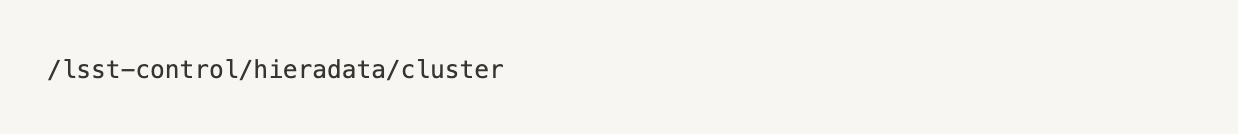
\includegraphics[width=12cm]{Images/Image2.png}
    \centering
\end{figure}
 

Once the folder is created contents should look like this and you should see the folder previously created along with YAML configurations files for various other nodes:
 
\begin{figure}
     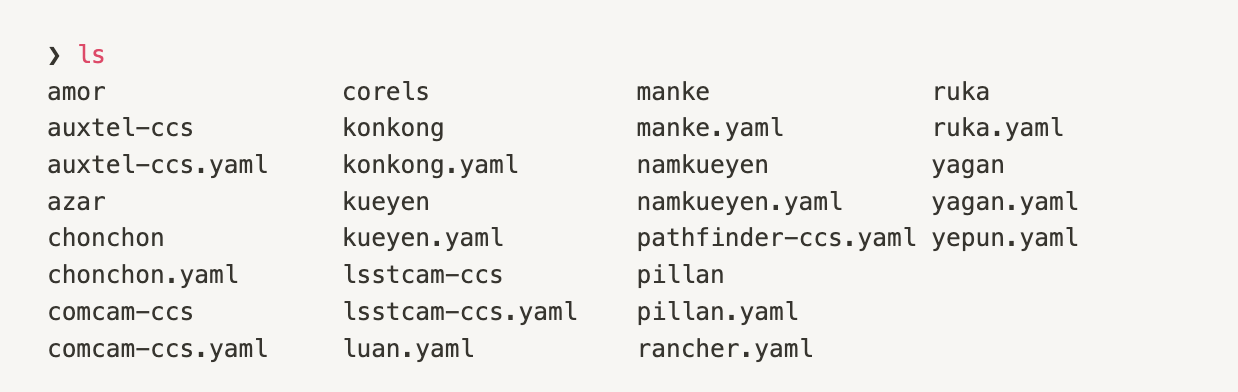
\includegraphics[width=12cm]{Images/Image3.png}
     \centering
\end{figure}

\vfill\eject

Create a YAML file for our nodes, this yaml file will store network specific configuration and will vary from host to host. Please adjust this template accordingly to meet your specific network configuration as interface naming conventions will change from one brand to another.


\begin{figure}
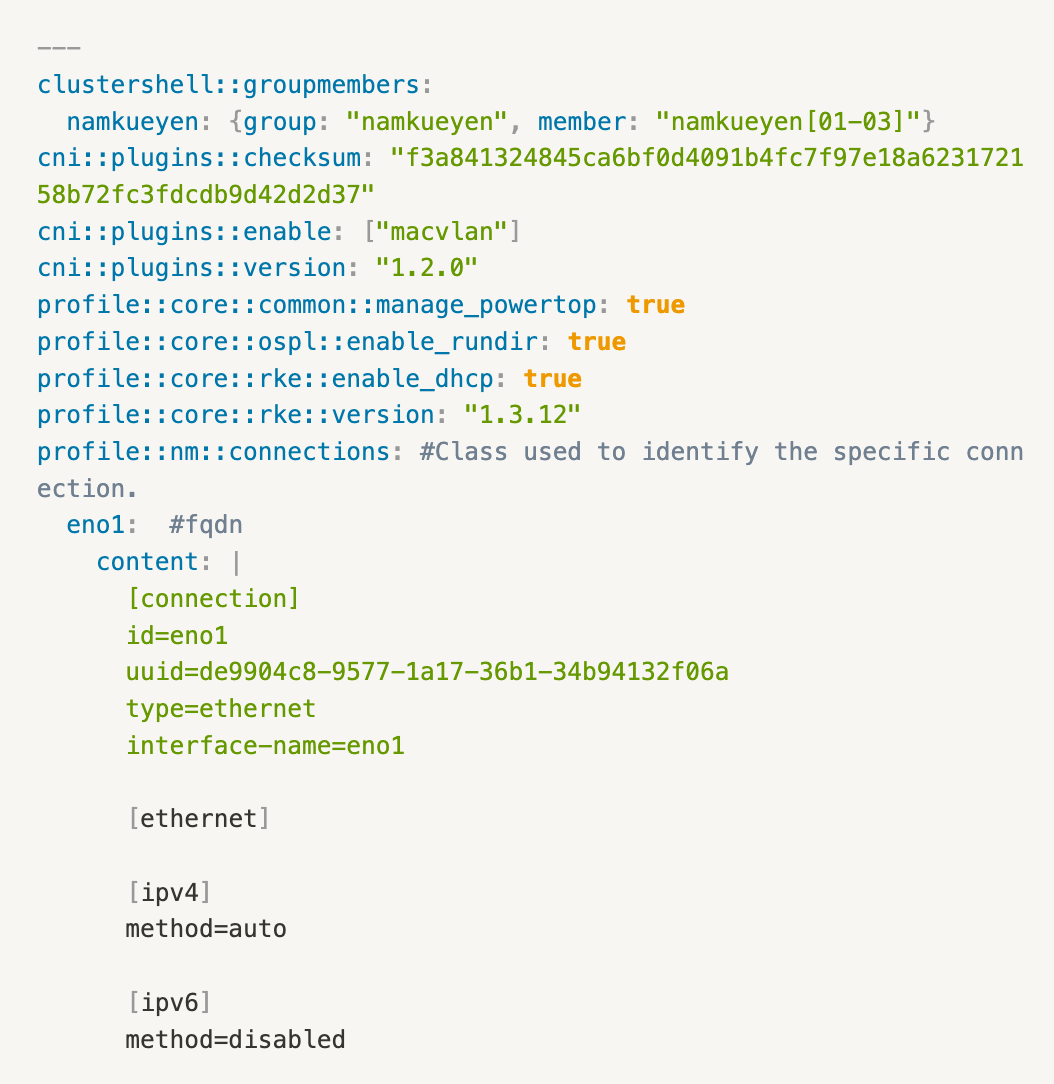
\includegraphics[width=12cm]{Images/Image5.png}
\centering
\caption{Example Network configuration file for Namkueyen Cluster Group}
\end{figure}

\vfill\eject


\subsection{LSST-Control / RKE Configuration}

Rancher Kubernetes Engine (RKE) is the tool responsible for initializing and managing our Kubernetes cluster.

\begin{itemize}
    \item Move inside the cluster folder previously created under /lsst/control/hierdata/cluster
    \item Inside this folder create a role folder.
    \item Inside the role folder create the rke.yaml configuration file using your editor of choice.
    \item In this step we can use another cluster rke configuration file as a template if necesary adjust it to your cluster specific needs and use.
\end{itemize}

\begin{figure}
    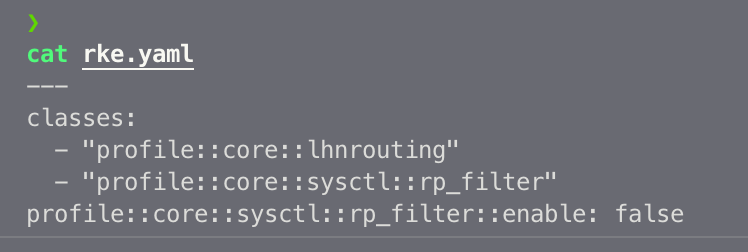
\includegraphics[width=12cm]{Images/Image9.png}
    \centering
    \caption{RKE Configuration Template Example}
    \end{figure}
    
\vfill\eject

\subsection{K8S Cookbook Repository}

The k8s-cookbook repository contains the recipes and notes for deploying our Kubernetes cluster.

\begin{itemize}
    \item First clone the repository on to your local enviroment. 
    \item Create a branch following the previous scheme, once this is complete create a cluster folder inside the k8s-cookbook folder.
\end{itemize}

Contents should look like this:

\begin{figure}
    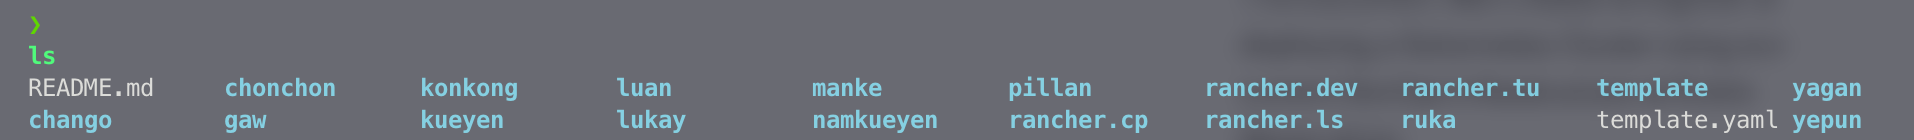
\includegraphics[width=12cm]{Images/Image10.png}
    \centering
    \caption{k8s-cookbook folder contents}
    \end{figure}


Inside our cluster folder, create the following folders, these folders will contain our Kuebrnetes deployment apps and scripts along with some instrucctions to properly execute them.

\begin{itemize}
    \item Cert Manager
    \item RKE
    \item Metallb
    \item Ingress
    \item rook-ceph
\end{itemize}

One the folders are created along with its contents please move on to the next step without executing the scripts as this will be done on a later stage of the deployment process.


\vfill\eject


\section{Foreman}

Foreman is a complete lifecycle management tool for physical and virtual servers. We'll be using it to manage our servers, so we need to set it up and configure it properly.

\subsection{Configuring and Provisioning the Server with Foreman}

Steps:

1. Log in to Foreman and head over to the discovered hosts tab and locate your server from the list.

\begin{figure}
    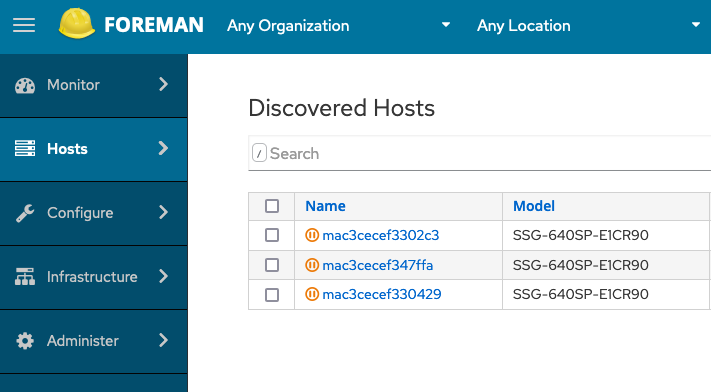
\includegraphics[width=12cm]{Images/Image11.png}
    \centering
    \caption{Discovered hosts}
\end{figure}

\vfill\eject

2. Once you have located the host, click the edit tab to configure the node.
\vspace{3cm}
\begin{figure}
    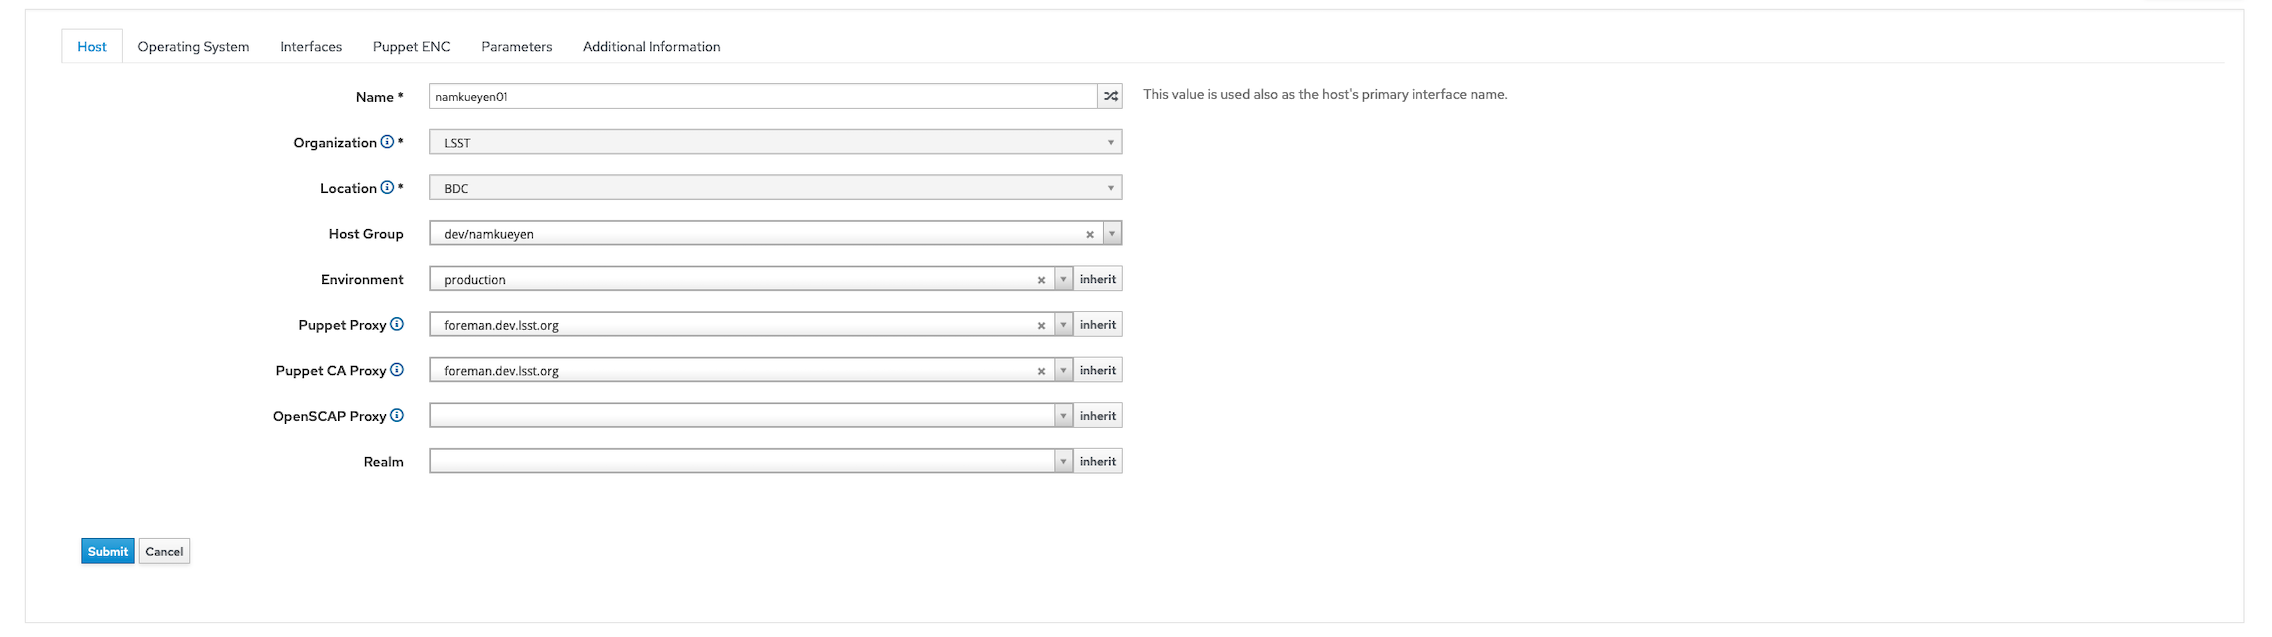
\includegraphics[width=14cm]{Images/Image12.png}
    \centering
    \caption{Configuration View}
\end{figure}

3. Select the OS the host will be provisioned with along with its respective partition table.
\vspace{3cm}
\begin{figure}
    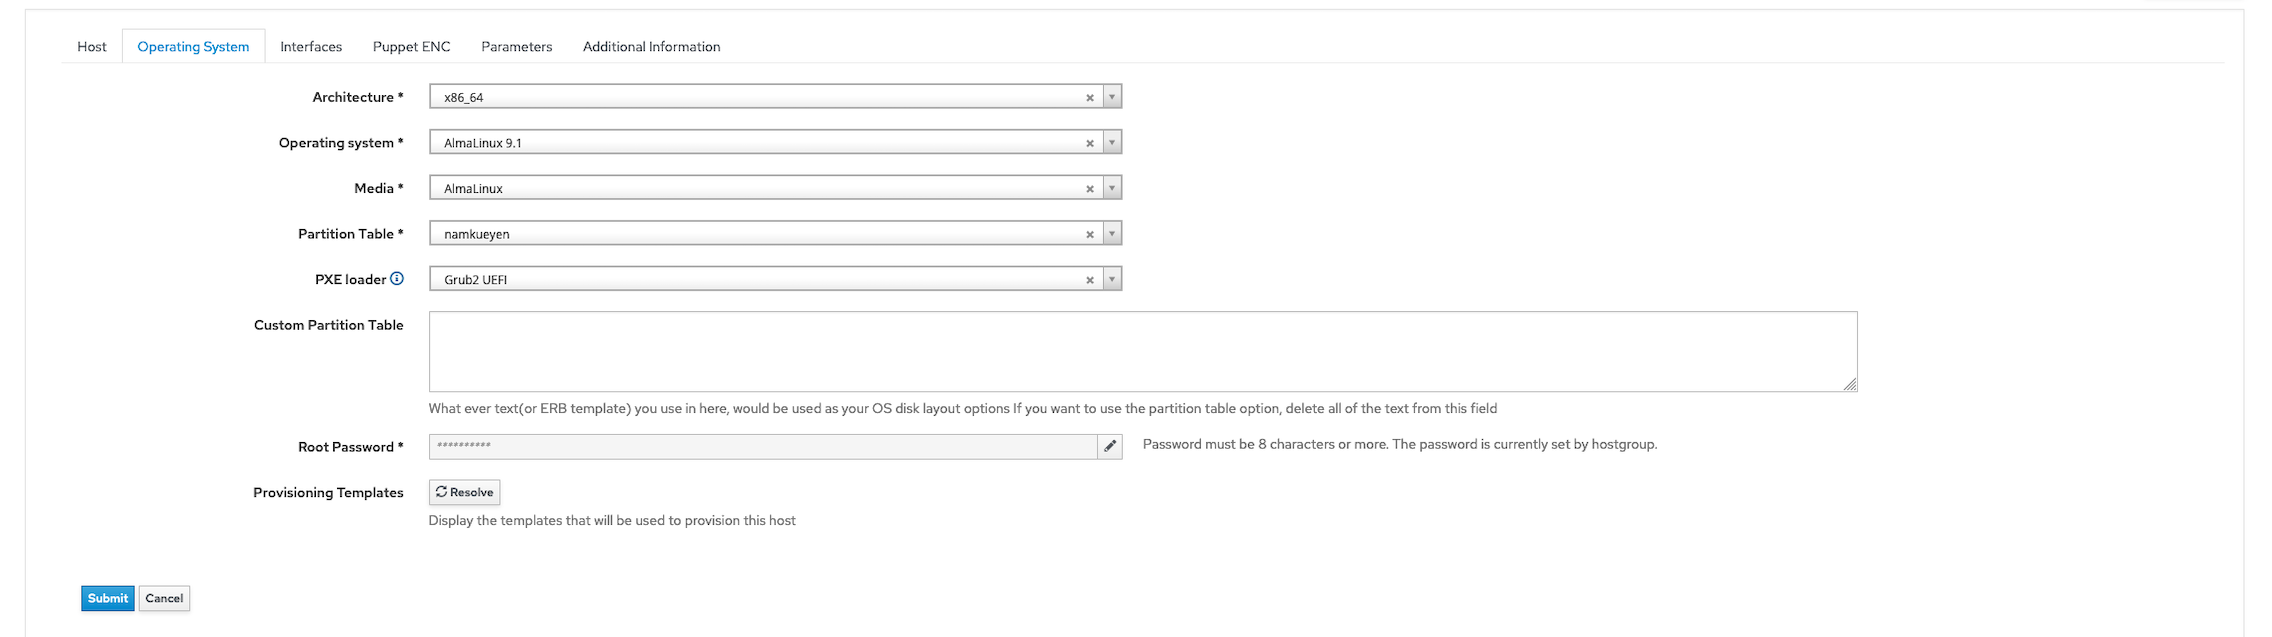
\includegraphics[width=14cm]{Images/Image13.png}
    \centering
    \caption{OS Configuration and Setup}
\end{figure}

\vfill\eject

4. Configure the nodes FQDN Interface and Management Interface in their respective subnets.
\vspace{0.5cm}
\begin{figure}
    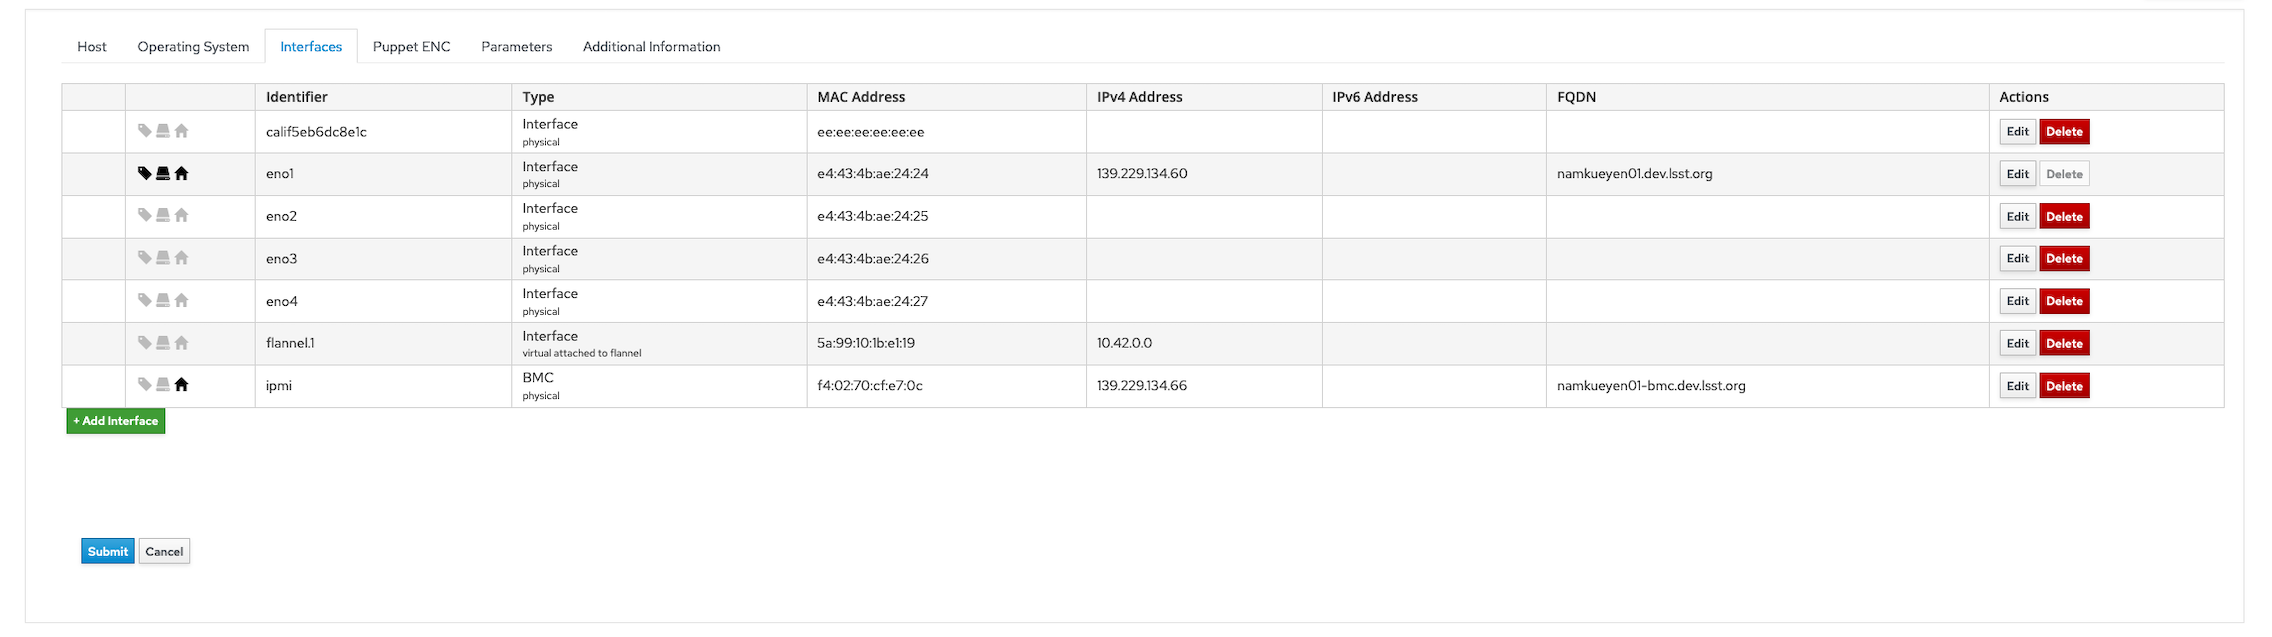
\includegraphics[width=12cm]{Images/Image14.png}
    \centering
    \caption{Network Configuration and Setup}
\end{figure}

\vspace{0.5cm}

5. Set the RKE role on the host along with FIPS enabled to False.

\begin{figure}
    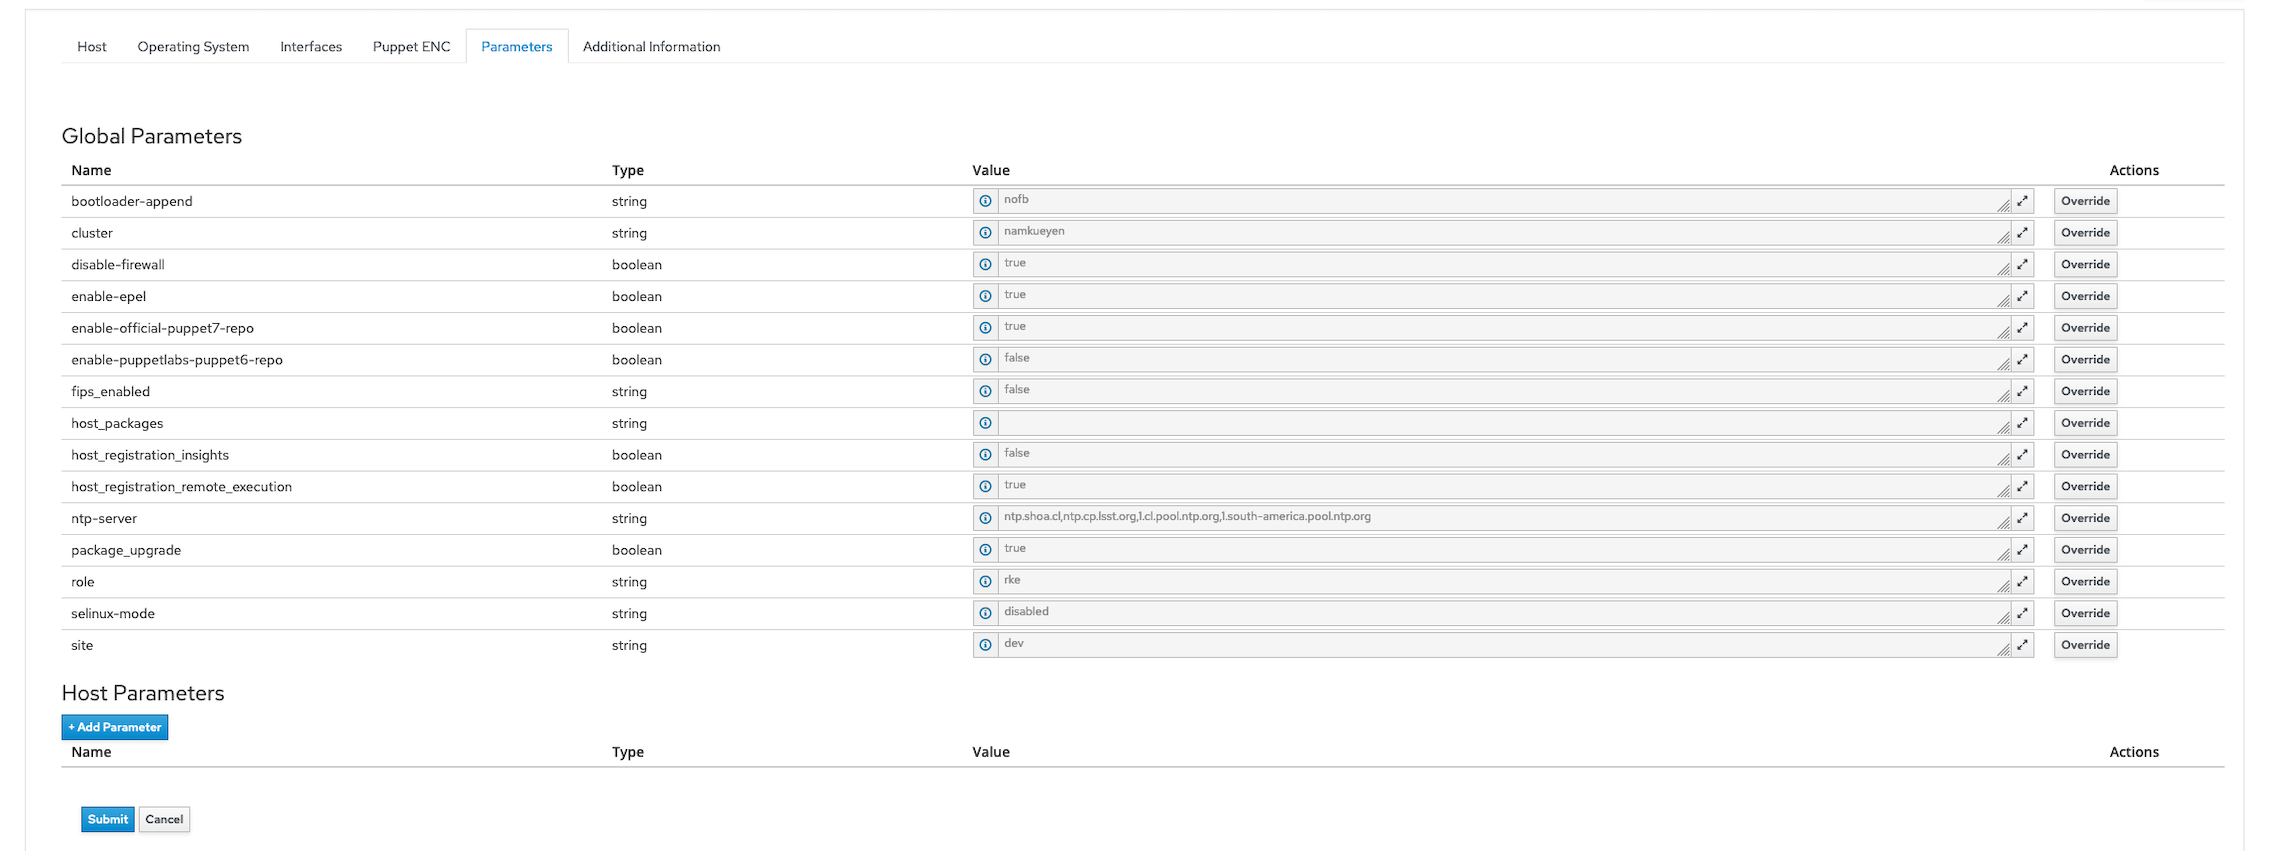
\includegraphics[width=12cm]{Images/Image15.png}
    \centering
    \caption{RKE Role and FIPS Setup}
\end{figure}


6. Once all is set up and configured proceed to provision the host and Run puppet once the OS is installed.

To run puppet:

\begin{center}
\begin{verbatim}
    puppet agent -t
\end{verbatim}
\end{center}

\begin{figure}
    
\includegraphics[width=12cm]{Images/Image16.png}
    \centering
    \caption{Node Provisioned}
\end{figure}

7. Repeat for the remaining nodes that compose the cluster group.

\vfill\eject

\section{Free IPA}
The Identity, Policy, Audit (IPA) is a project providing an open-source identity management solution. It's important to ensure that the hosts are in IPA, as this allows for proper authentication, authorization, and auditing.

\subsection {Setup and Configuration of Cluster Group in IPA}

1. Check that the cluster group nodes show up on IPA under the hosts tab.

\begin{figure}
    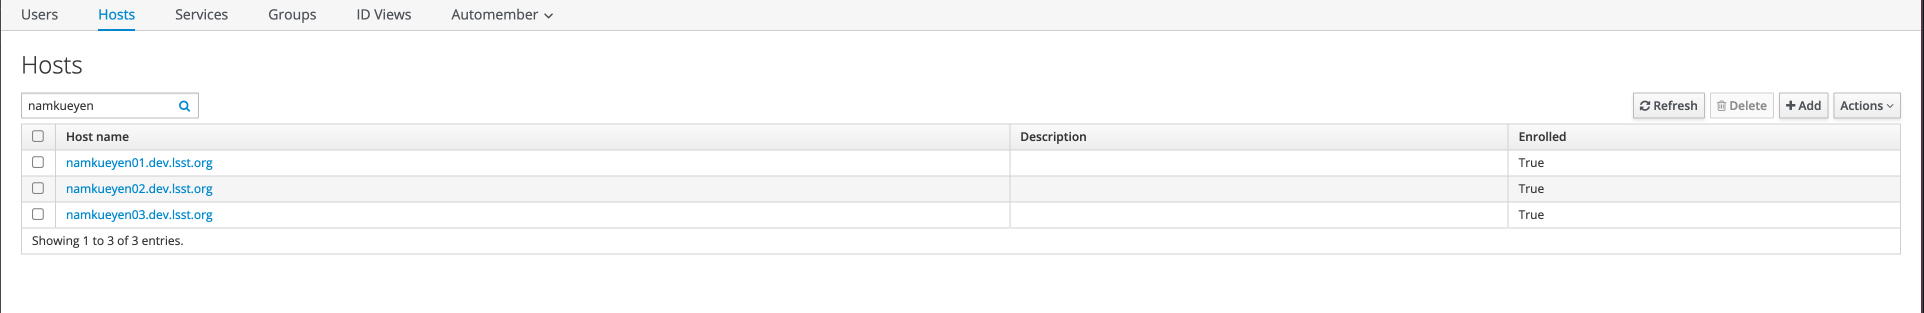
\includegraphics[width=12cm]{Images/Image17.png}
    \centering
    \caption{Hosts}
\end{figure}

2. Create a user cluster group and a user sudo group under the Groups tab on IPA.

\begin{figure}
    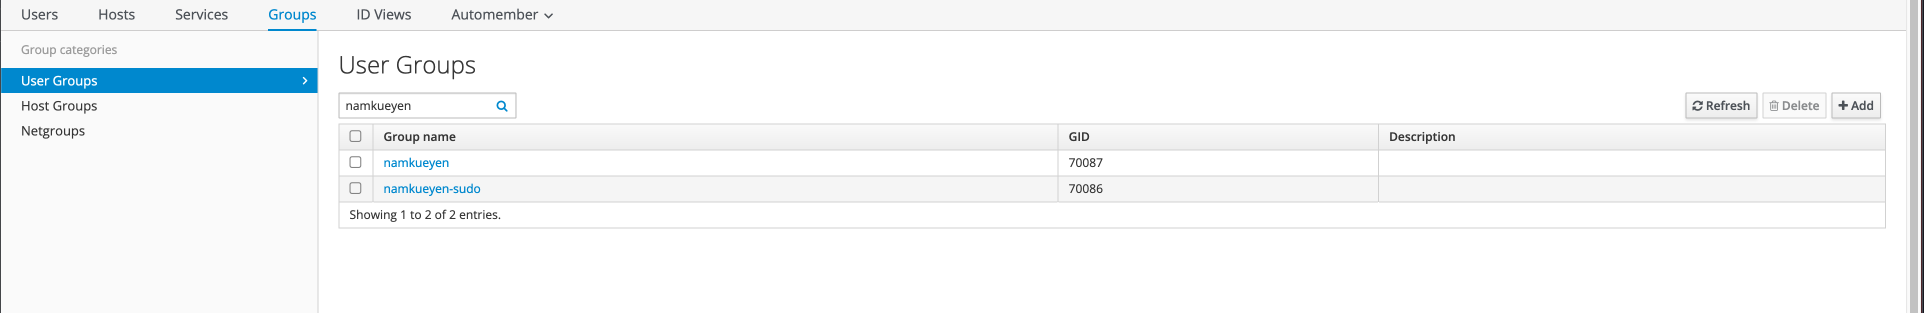
\includegraphics[width=12cm]{Images/Image19.png}
    \centering
    \caption{User Group Creation}
\end{figure}

2.1 Under the user group just created add the rke user to the cluster group.

\begin{figure}
    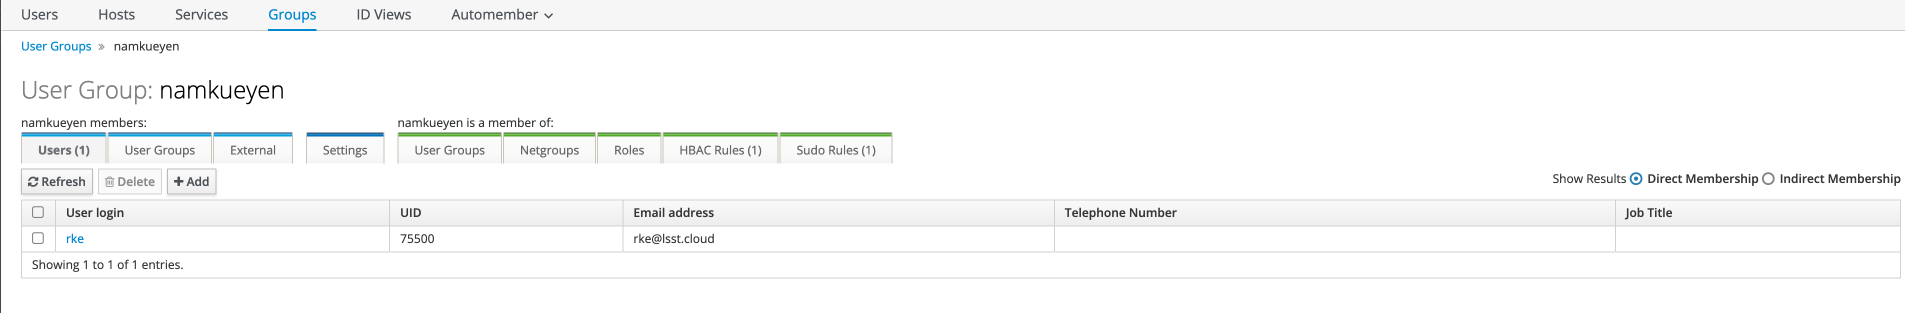
\includegraphics[width=12cm]{Images/Image21.png}
    \centering
    \caption{Add RKE User to User Group}
\end{figure}


3. Create a cluster host group and add the cluster group nodes to the host group. 

\begin{figure}
    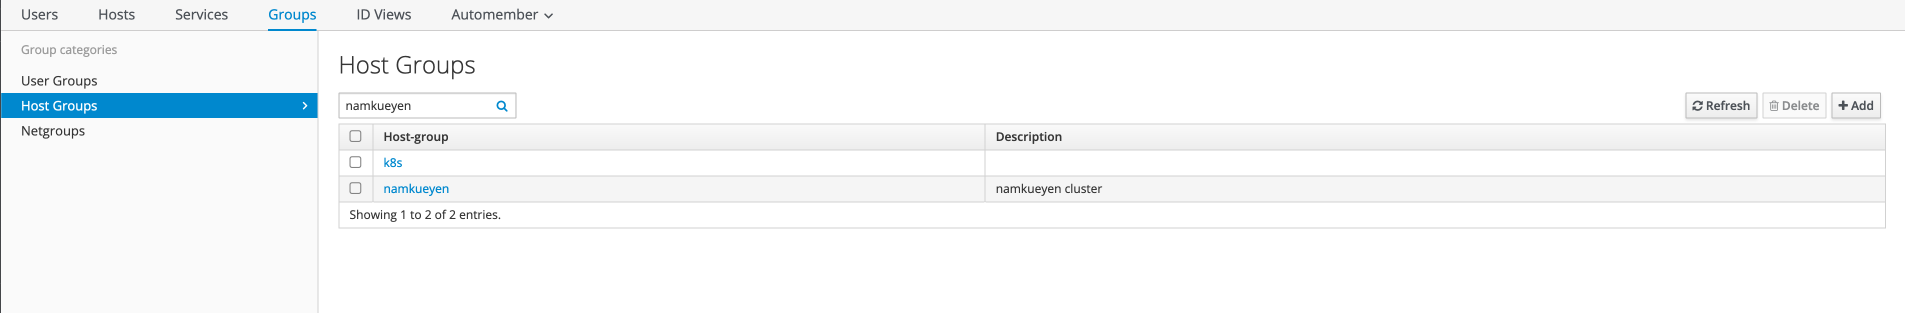
\includegraphics[width=12cm]{Images/Image20.png}
    \centering
    \caption{Host Group Creation}
\end{figure}

4.  Add the Namkueyen host group to the k8s group on IPA.

\begin{figure}
    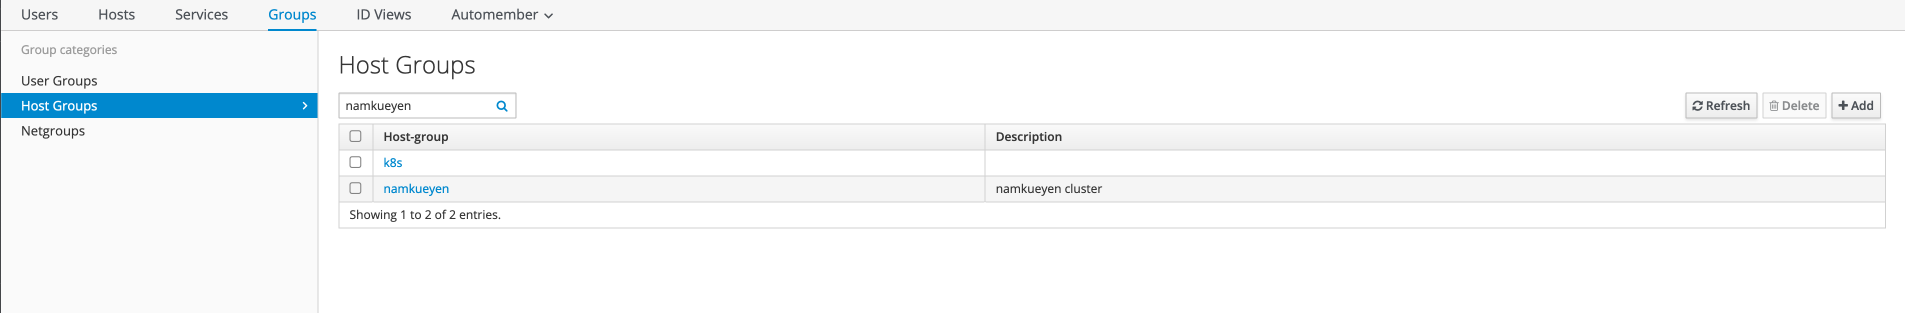
\includegraphics[width=12cm]{Images/Image20.png}
    \centering
    \caption{Add Host group to K8S group on IPA}
\end{figure}

5. Creating a Host Based Access Control Rule for the user group and host group.

\begin{figure}
    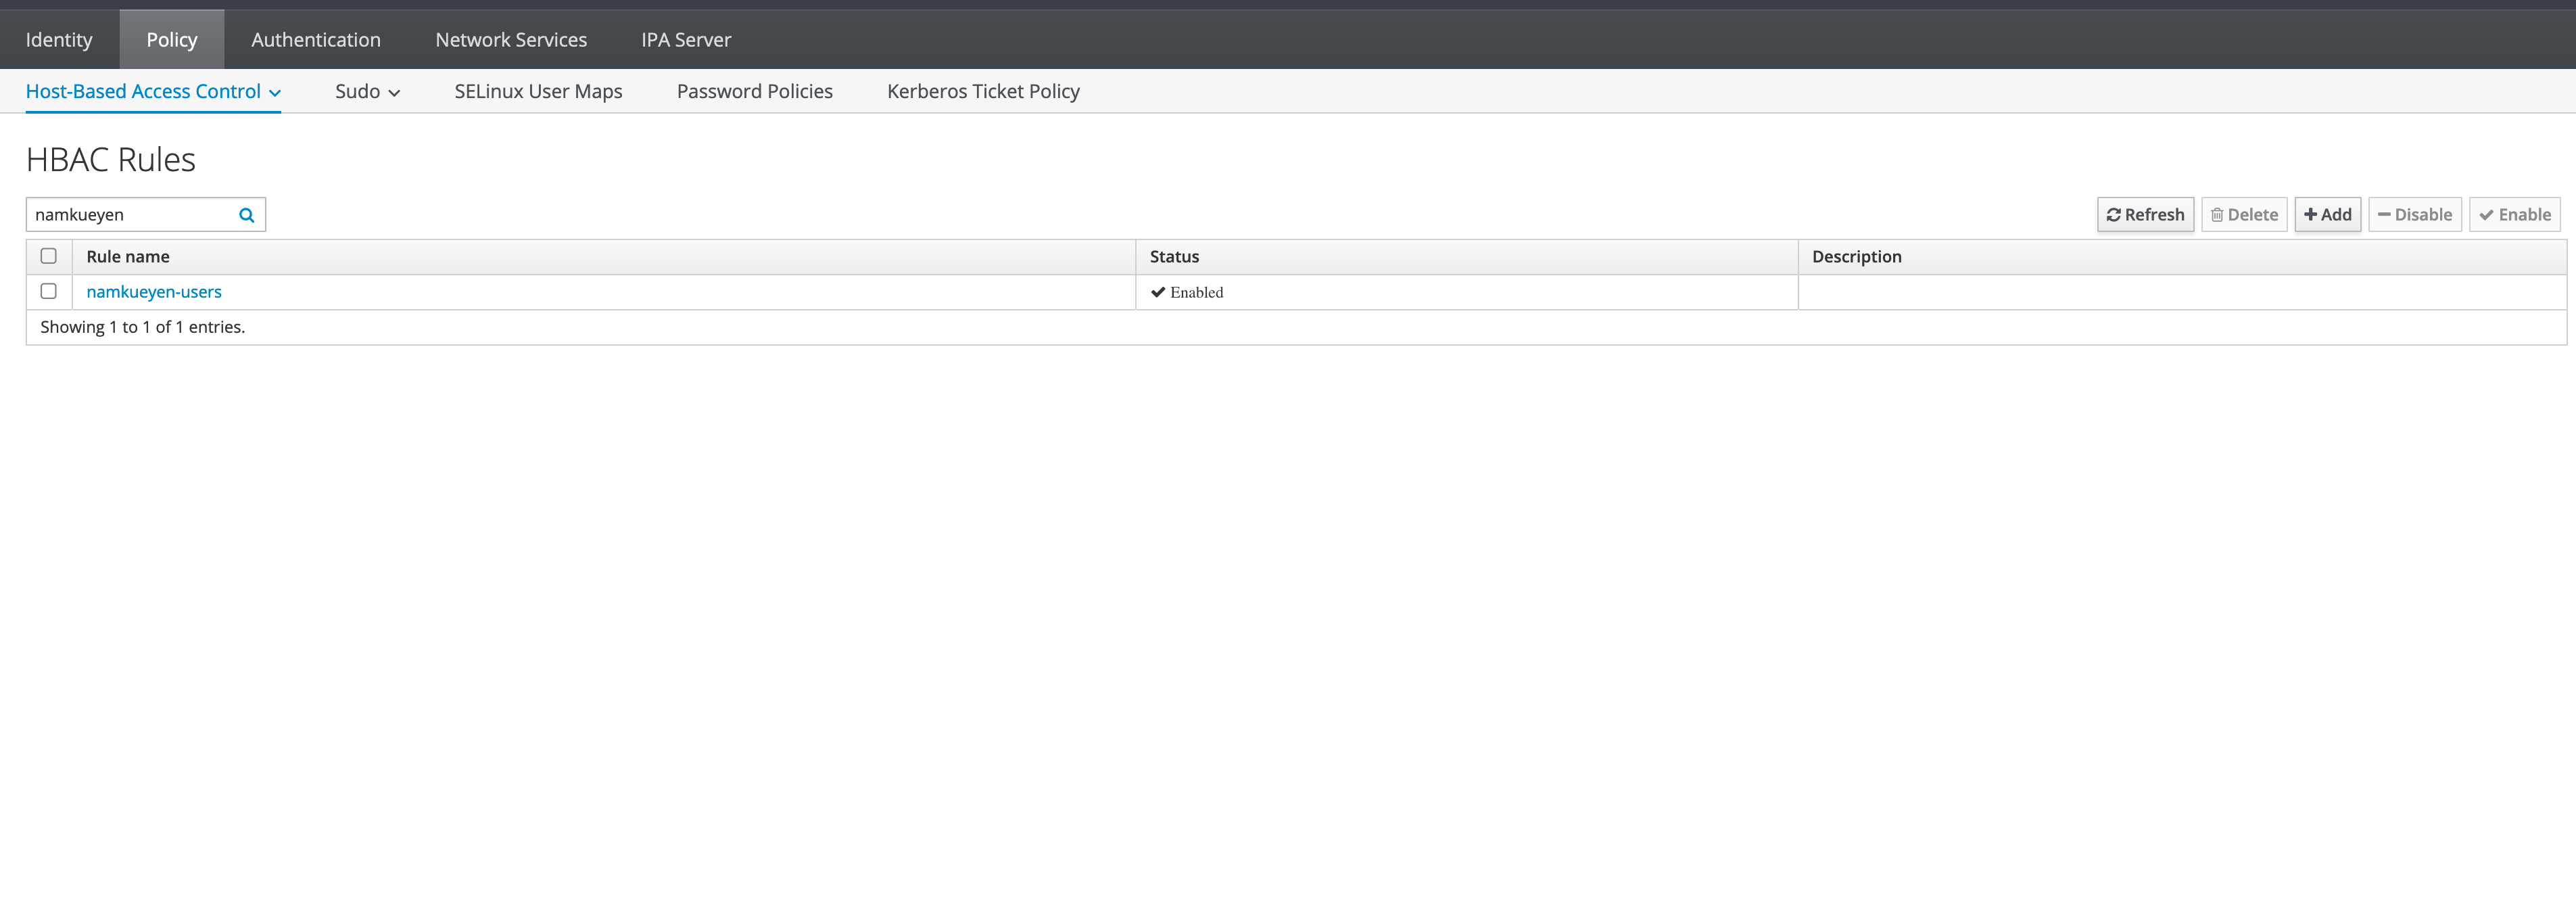
\includegraphics[width=12cm]{Images/Image23.png}
    \centering
    \caption{Creating an HBAC Rule}
\end{figure}

5.1 Configuring the HBAC Rule properties.

\begin{figure}
    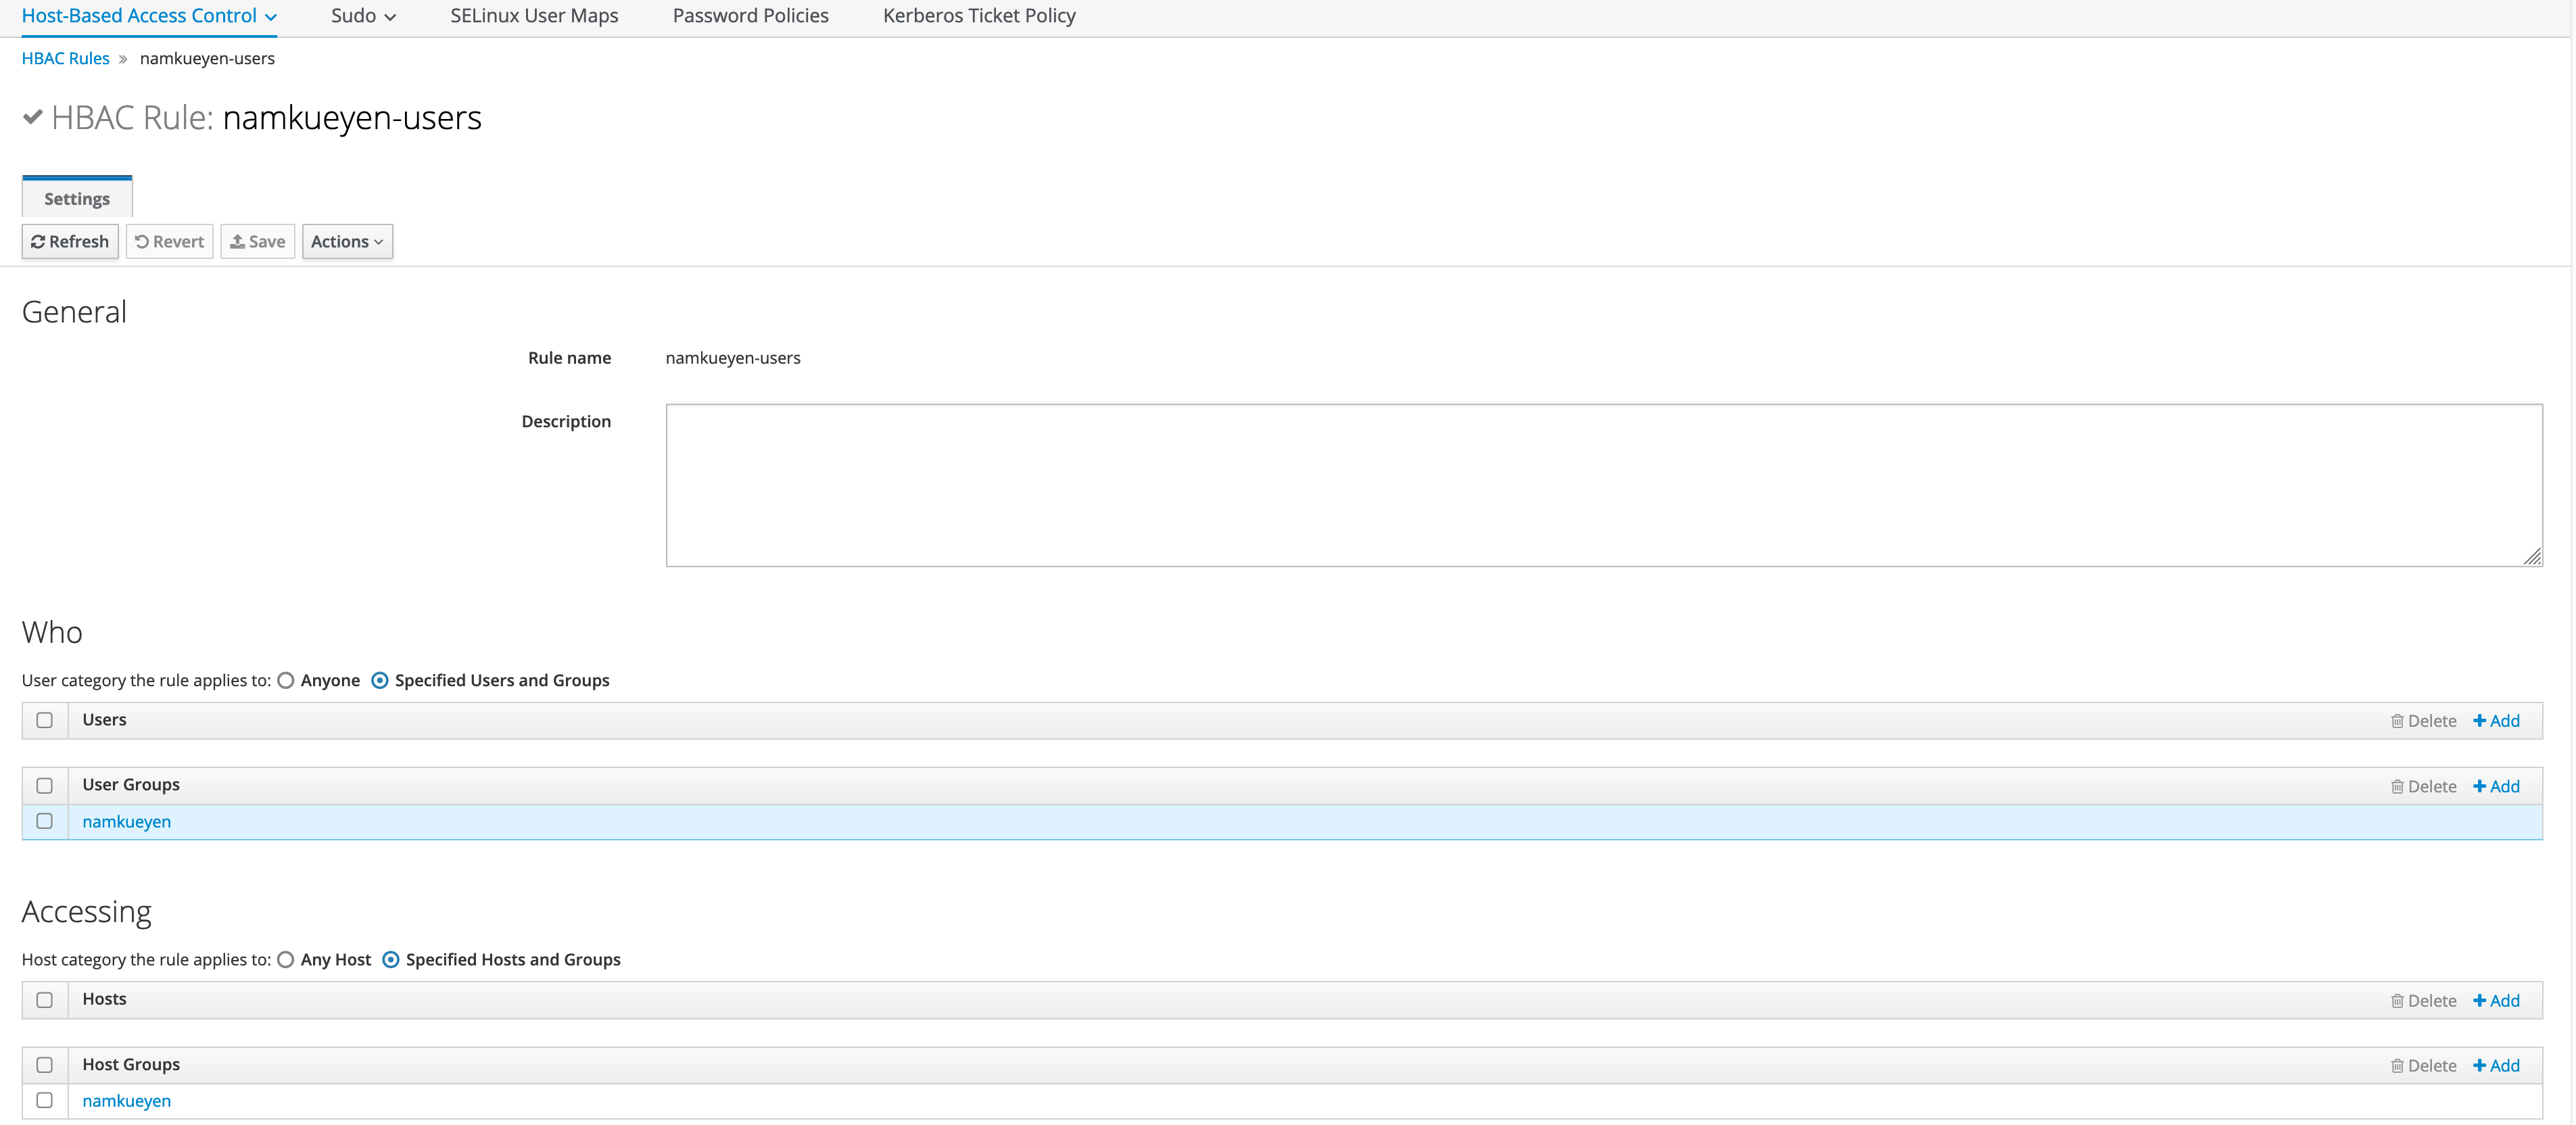
\includegraphics[width=12cm]{Images/Image24.png}
    \centering
    \caption{HBAC Rule Properties Setup}
\end{figure}

\vfill\eject

6. Creating a Sudo Rule for the user group and host group previously created. 

\begin{figure}
    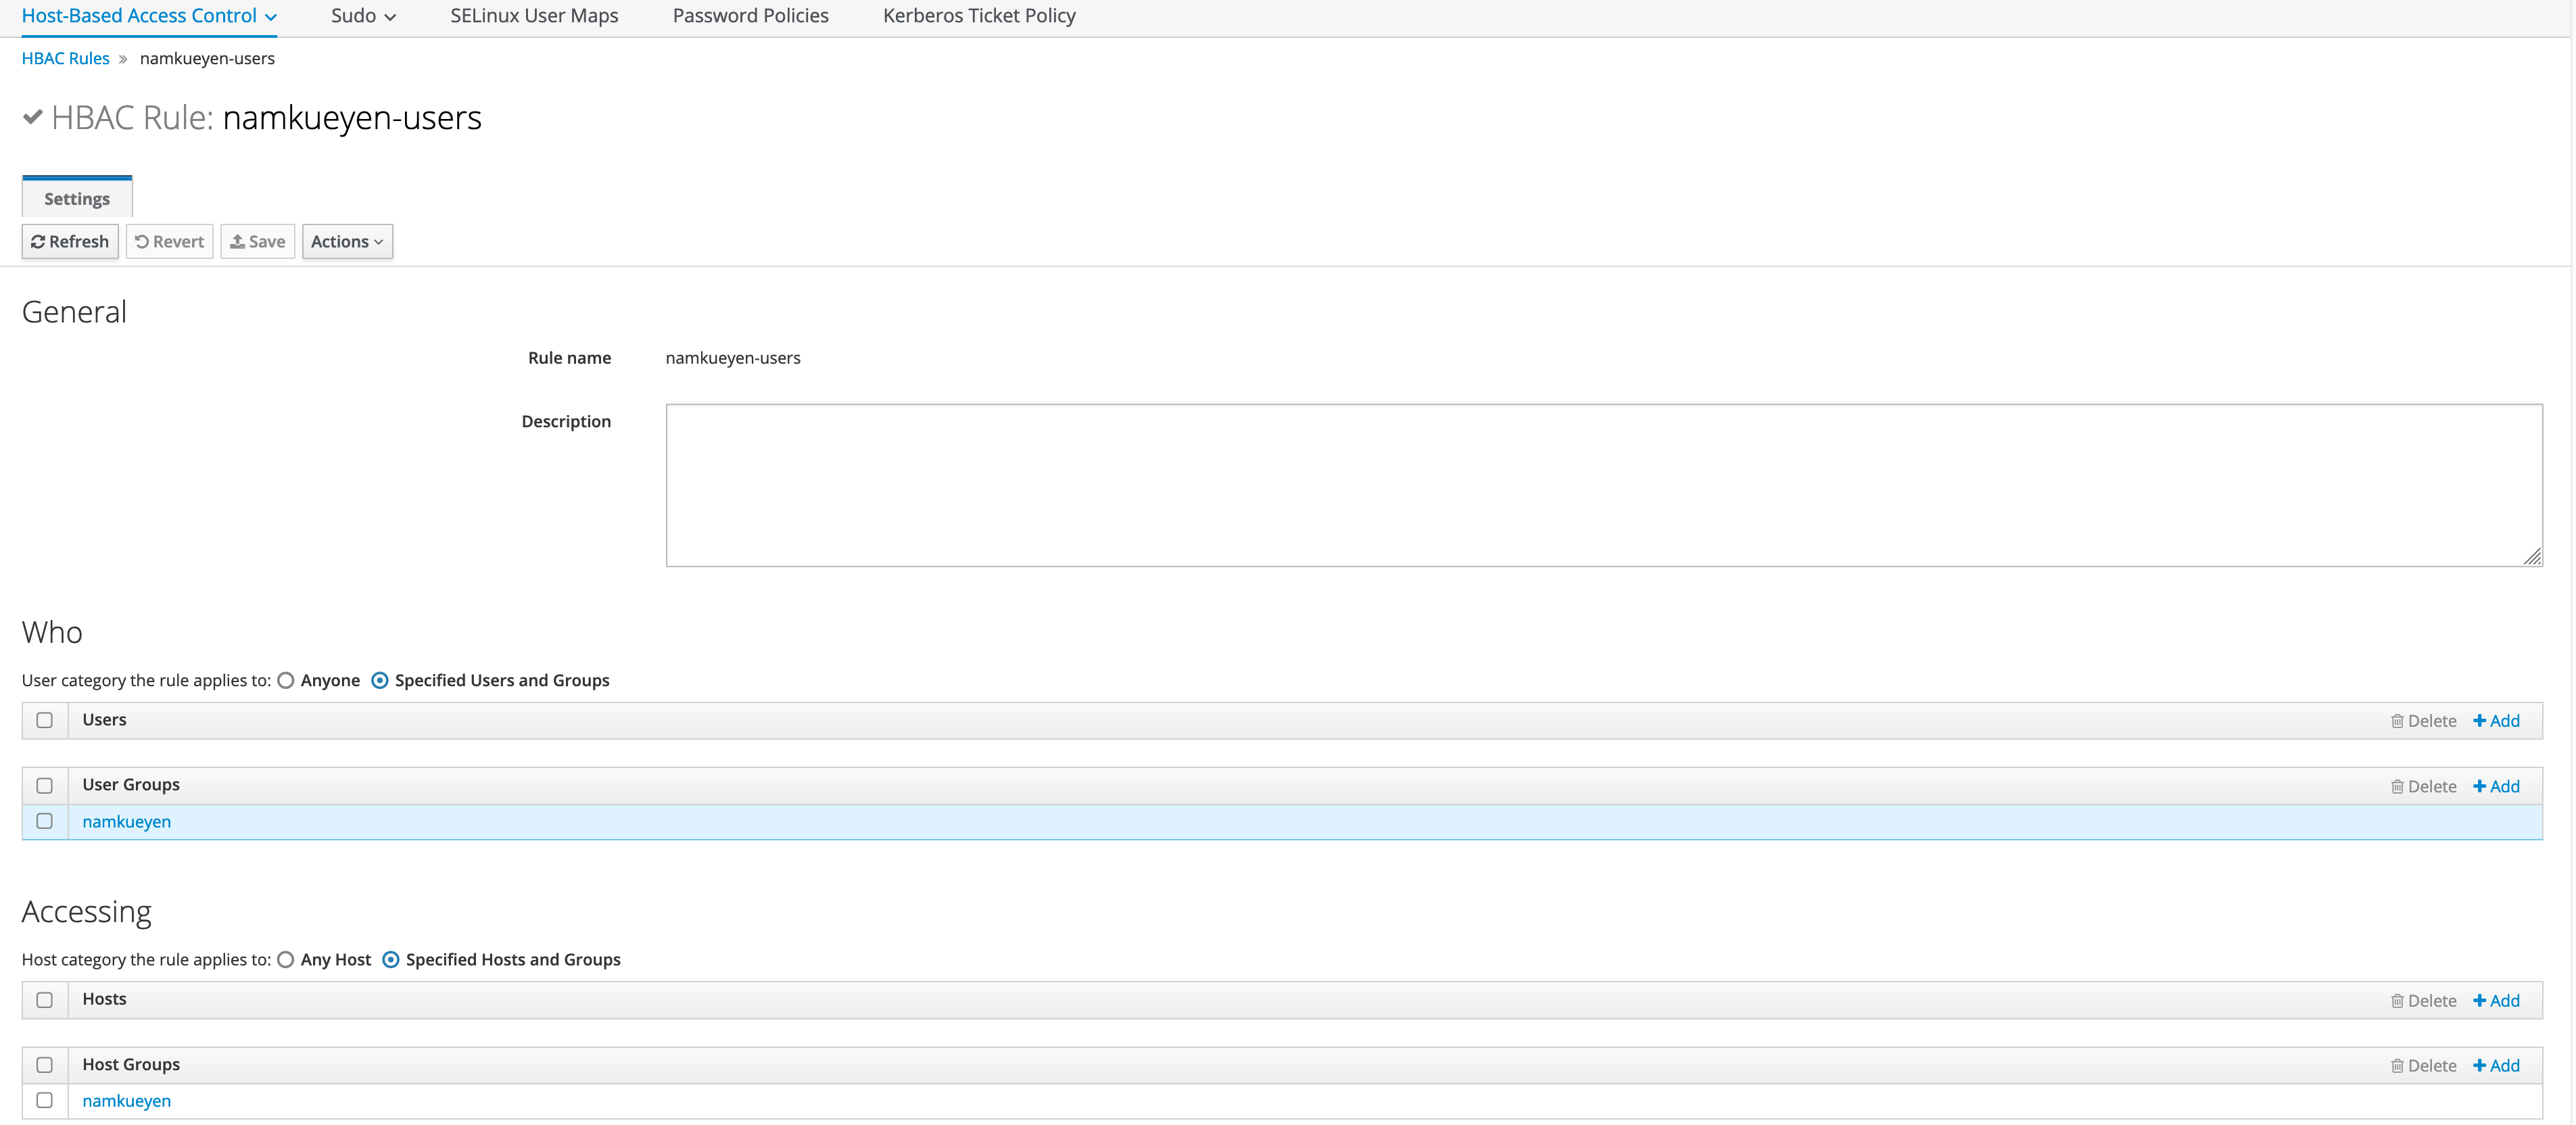
\includegraphics[width=12cm]{Images/Image24.png}
    \centering
    \caption{Sudo Rule Creation}
\end{figure}


6.1 Add the groups to which these rules will apply to along with the hosts which these rule will take effect.

\begin{figure}
    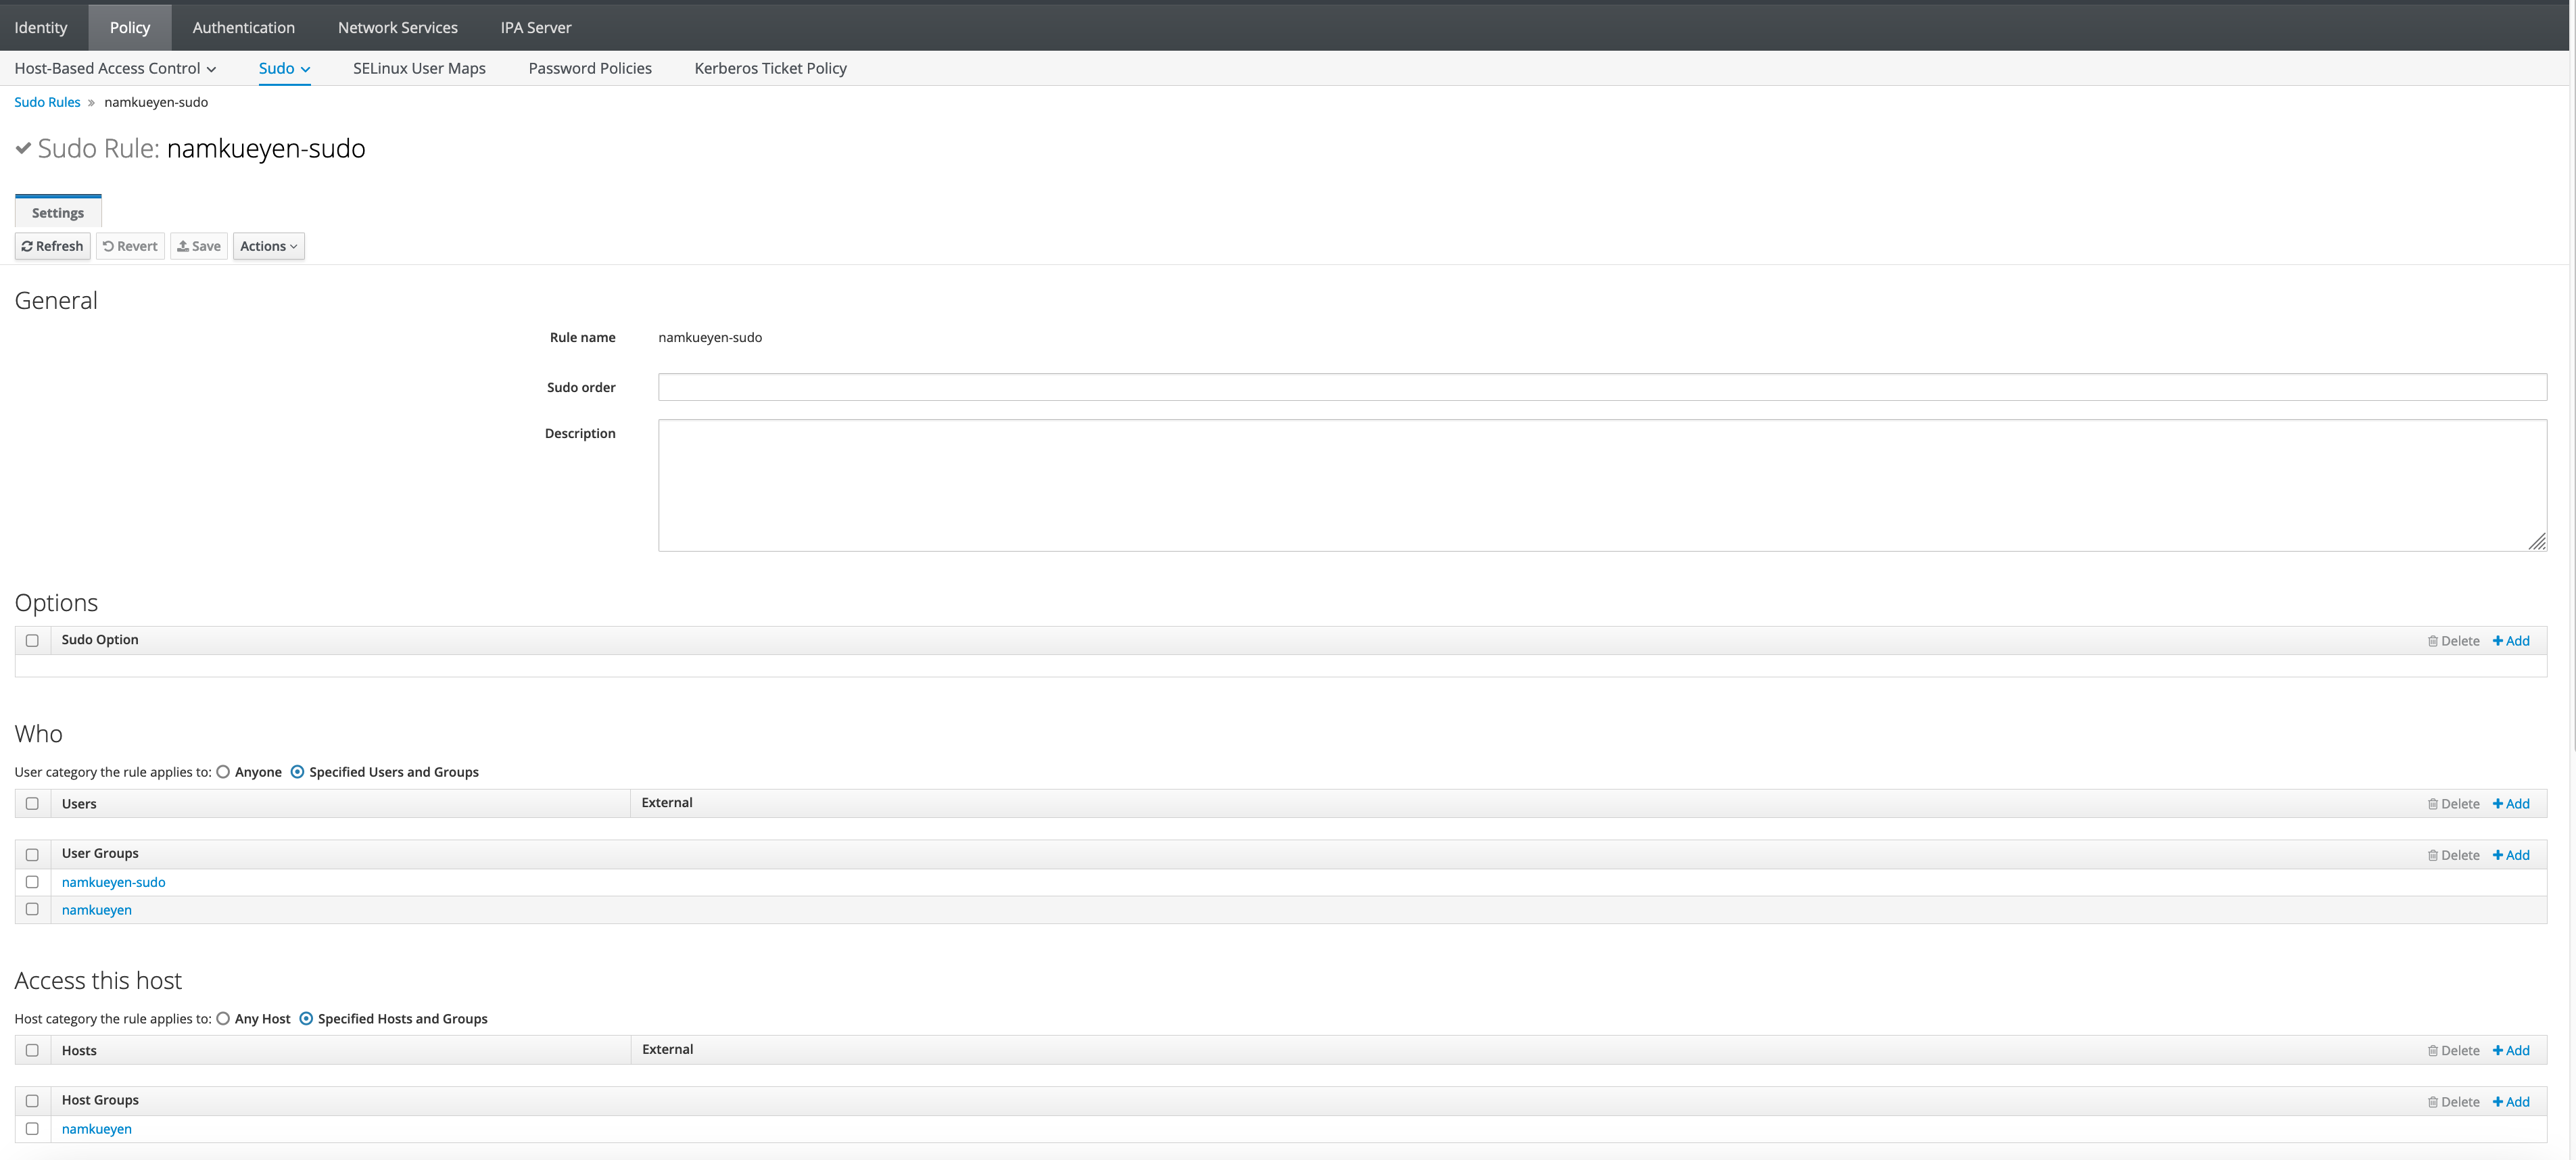
\includegraphics[width=12cm]{Images/Image26.png}
    \centering
    \caption{Sudo Rule Creation}
\end{figure}

7. Lastly create a Automember host group rule.

\begin{figure}
    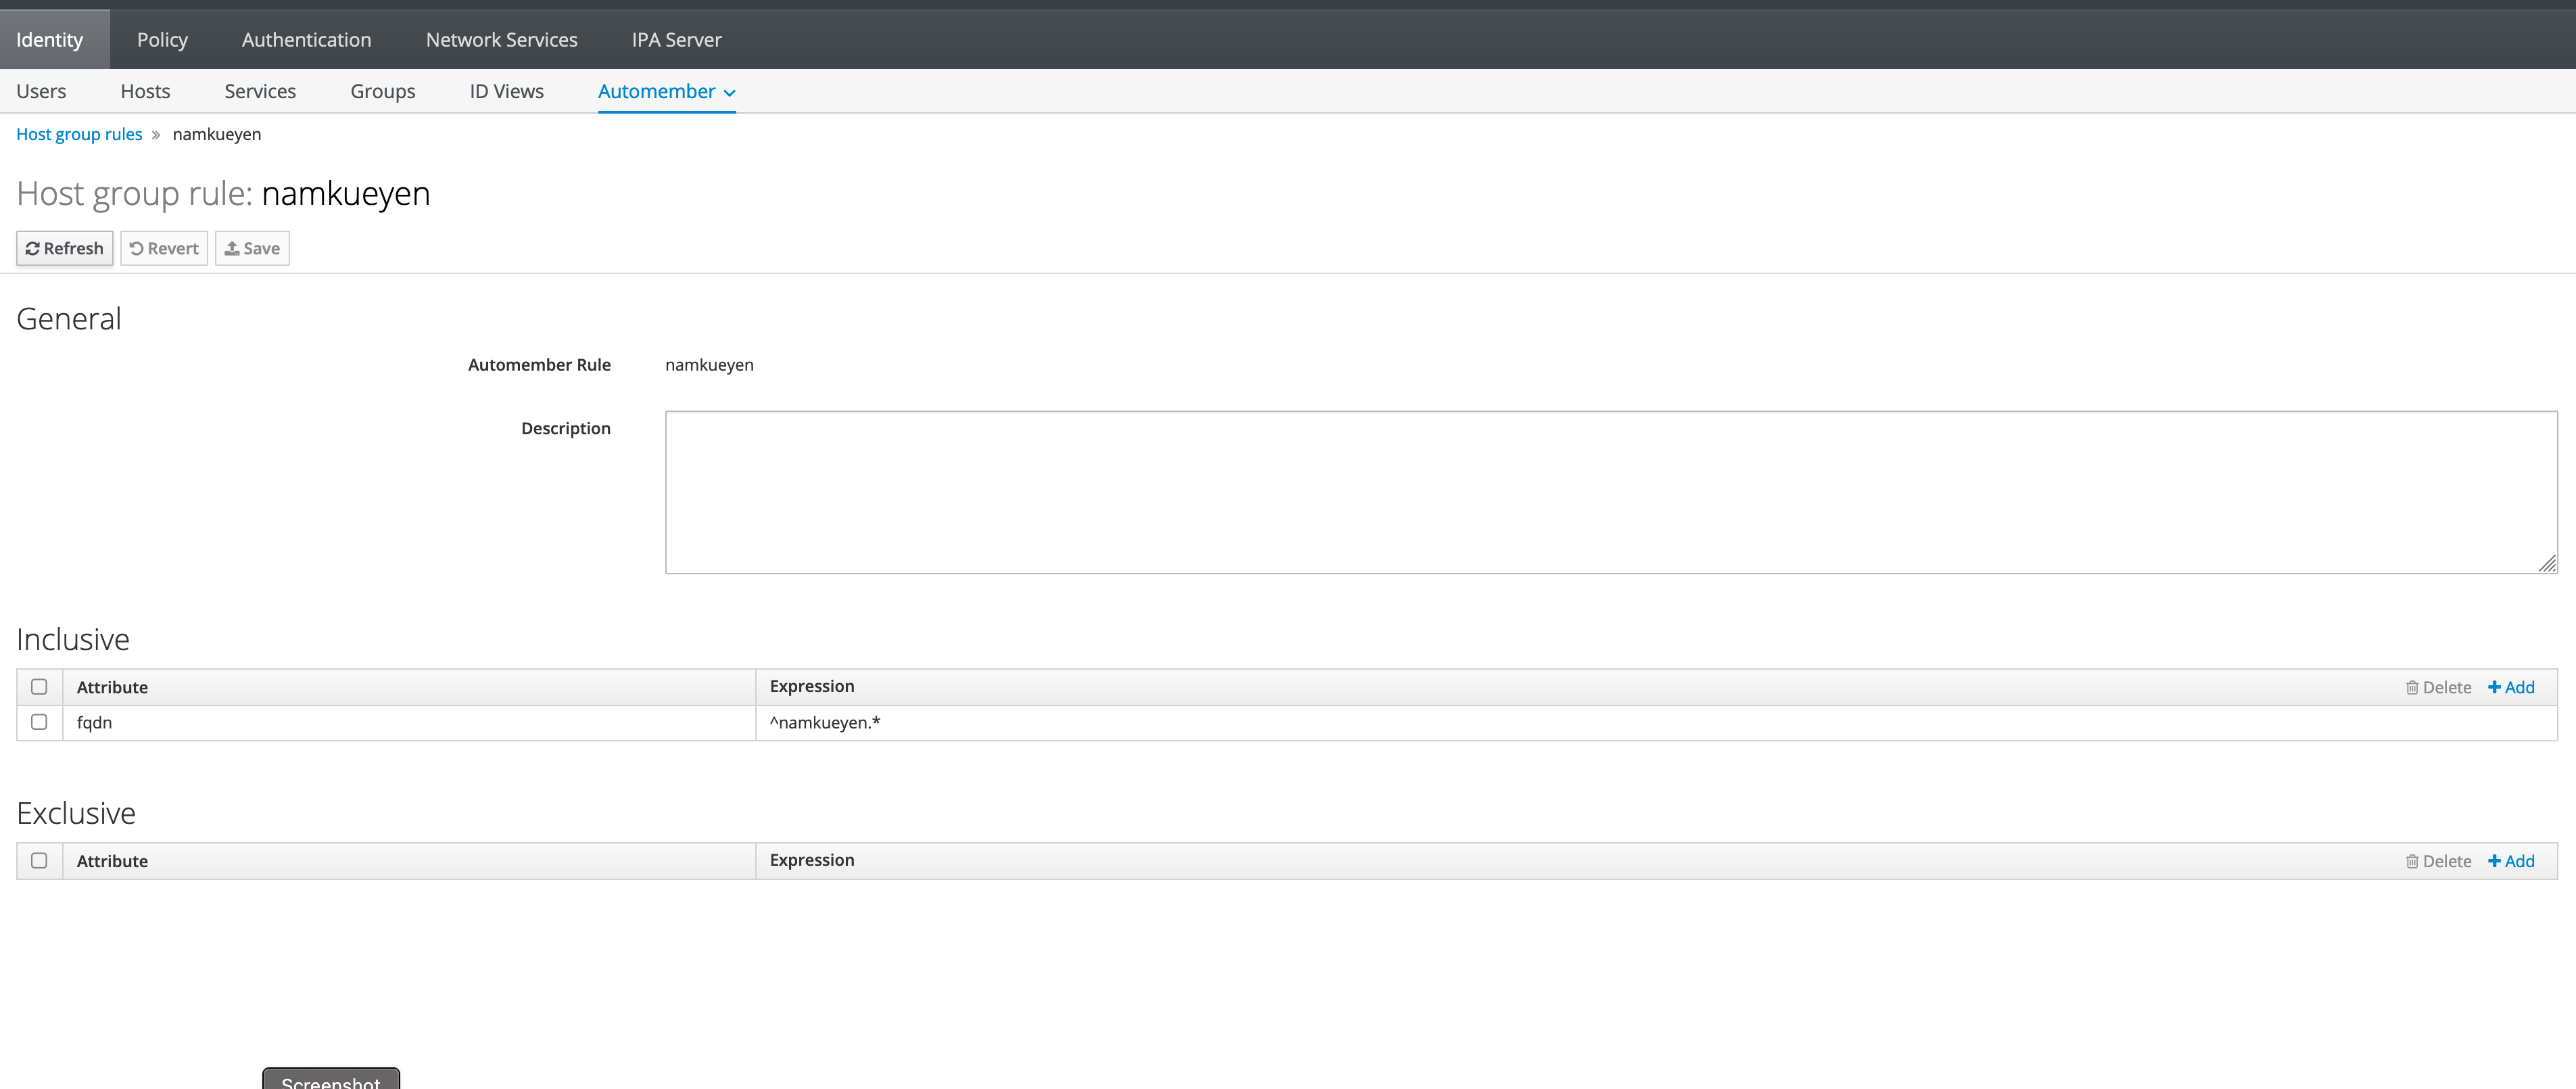
\includegraphics[width=12cm]{Images/Image27.png}
    \centering
    \caption{Automember Rule Creation}
\end{figure}



\vfill\eject

\section{Testing Connectivity Between Nodes}
Before deploying the cluster, it's crucial to test the connectivity between nodes. This step ensures that the nodes can communicate with each other, which is essential for the functioning of the Kubernetes cluster.

\vfill\eject

\section{RKE Cluster Build}
With all the configurations and testing done, we can now build our RKE cluster. This step involves running the RKE command to bring up the cluster.

\vfill\eject

\section{Executing Deployment Scripts}
Finally, execute the deployment scripts. These scripts automate the process of deploying the Kubernetes cluster, saving time and reducing the possibility of errors. The deployment scripts to be executed are for the various services that will run in our cluster. These services include:

\begin{itemize}
    \item CertManager: Manages certificate issuance in the cluster, enabling secure communication between services.
    \item Metallb: Provides load-balancing for our services, helping to distribute network traffic for better performance and reliability.
    \item Ingress: Manages external access to the services in the cluster, acting as a router for incoming requests.
    \item Rook-ceph: Provides storage solutions for our cluster, enabling persistent storage for our services.
\end{itemize}